\subsubsection{Cube ou continuation}
Cet opérateur a été créé pour être une réponse efficace à nos problèmes.
%
Dans notre cas, le graphe à ordonnancer à exactement la même structure que le réservoir que nous souhaitons modéliser.
%
La plupart du temps, ce modèle sera un cube 3D.
%
En numérotation naturelle et avec un modèle 3D, une bonne agrégation consiste à agréger toutes les tâches d'un axe qui ont les mêmes coordonnées sur les deux autres axes.
%
Ca correspond à {\em aplatir} notre modèle 3D en un modèle 2D (Fig.~\ref{fig:cube5_algo_C}).
%
Par exemple, un cube de 5 éléments de coté, soit 125 tâches, sera transformé en un carré de 5 éléments de coté, soit 25 tâches.


%   (-_-)   %
\begin{figure}[t!]
  \centering
  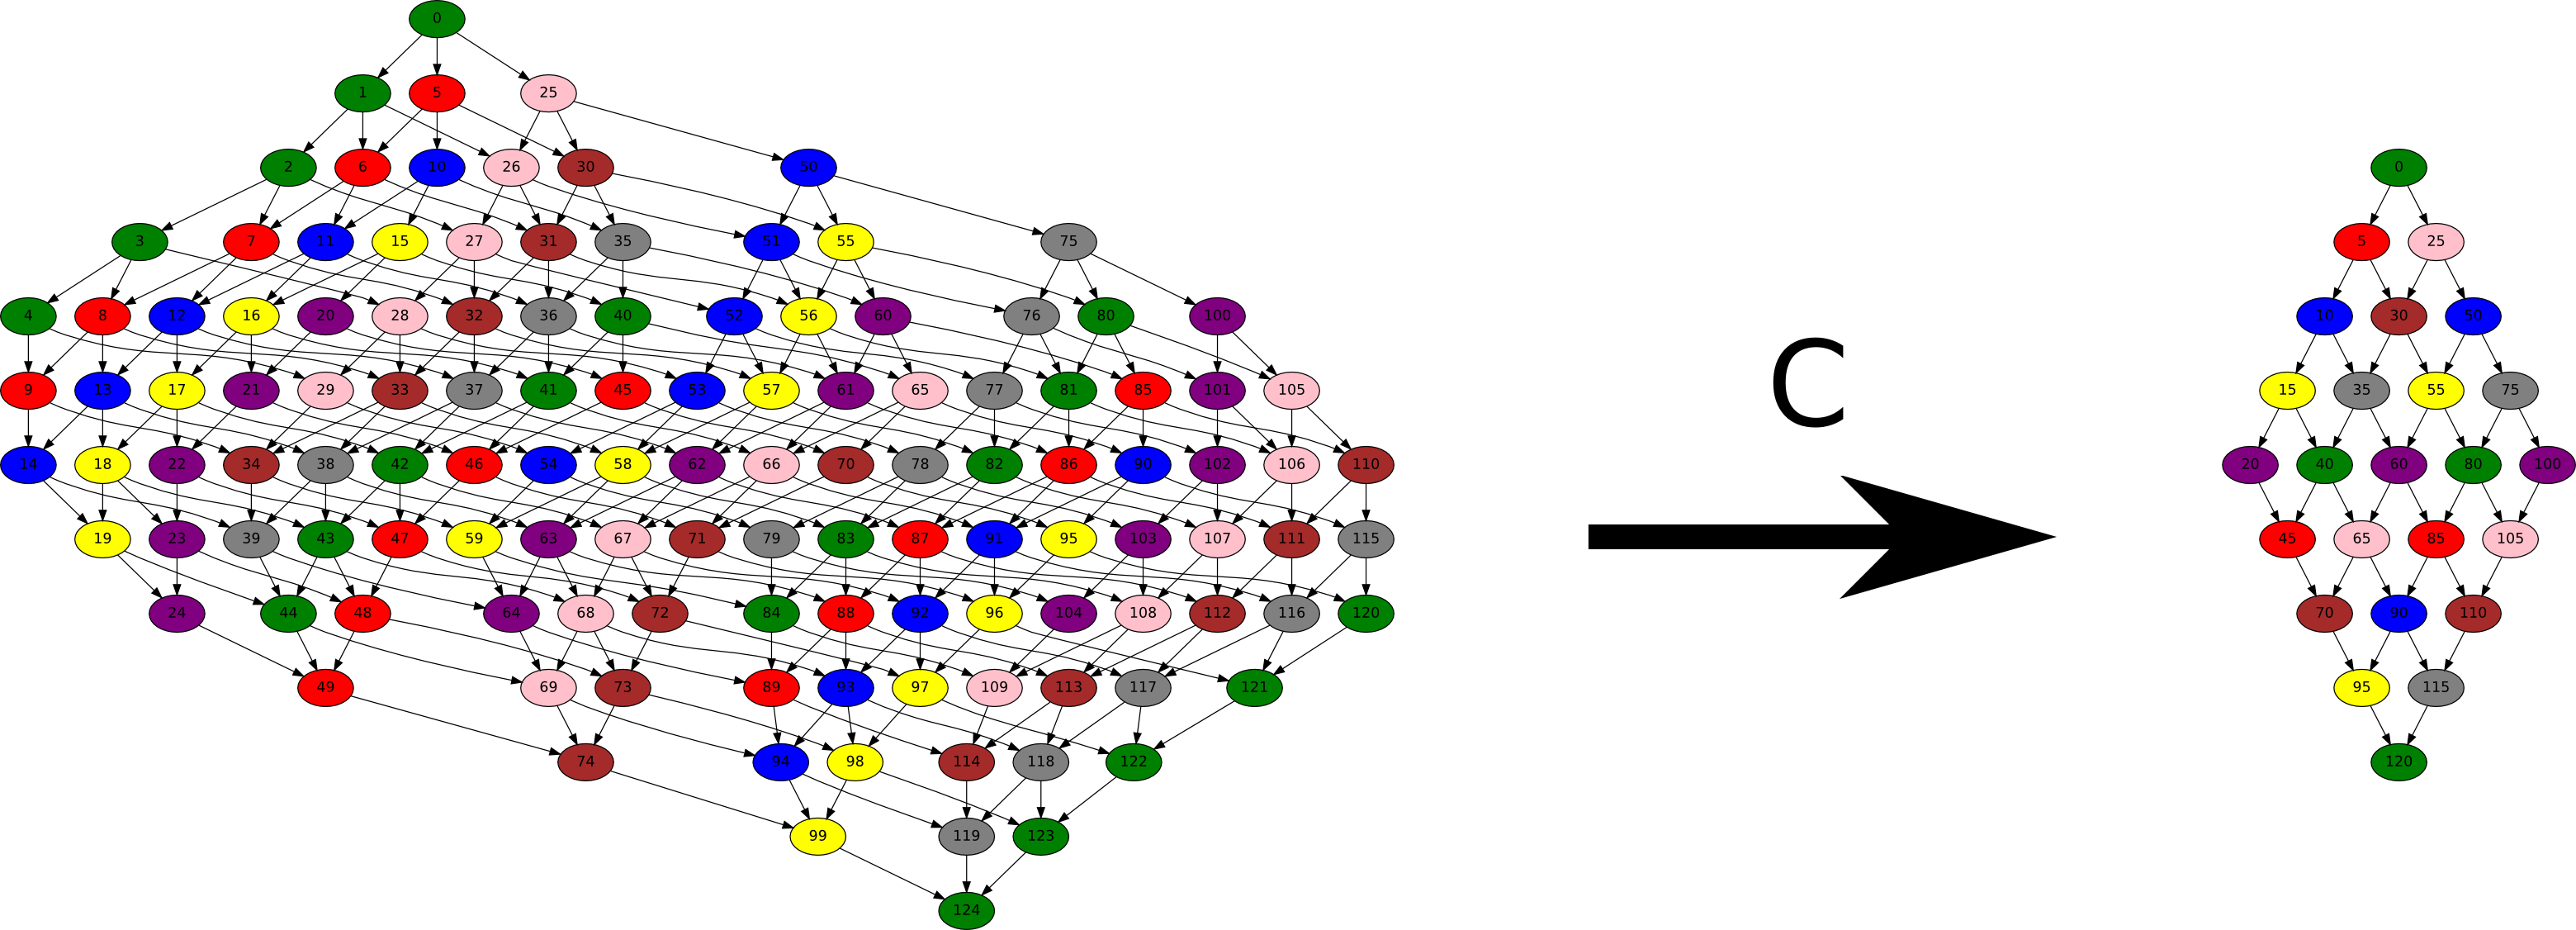
\includegraphics[width=\textwidth]{cube5_operator_c}
  \caption{Exemple d'utilisation de l'opérateur C sur un cube 5x5x5.}
  \label{fig:cube5_algo_C}
\end{figure}


%   (-_-)   %
\begin{figure}[t!]
  \centering
  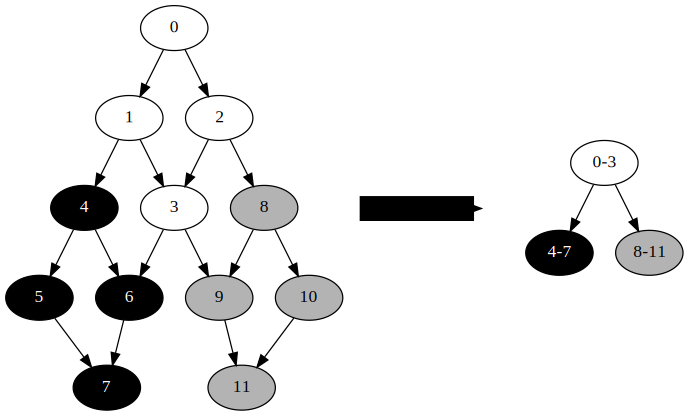
\includegraphics[width=0.8\textwidth]{algo_3}
  \caption{Exemple d'utilisation de l'opérateur C.}
  \label{fig:algo_C}
\end{figure}


Comme pour les autres opérateurs, nous devons vérifier qu'aucun cycle ne sera créé.
%
Pour fonctionner, cet opérateur a besoin que le programmeur attribut un nombre unique à chaque tâche et ainsi avoir un ordre strict sur les tâches.
%
Dans notre cas on va utiliser la numérotation naturelle.
%
Puis l'opérateur agrégera ensemble les tâches ayant des nombres qui se suivent ainsi qu'une dépendance entre les tâches.

Ajoutons un prédicat à l'algorithme : pour pouvoir utiliser cet algorithme, il faut absolument que pour chaque tâche $i$, l'indice associé à la tâche $i$ soit strictement inférieur aux indices associés aux successeurs de la tâche $i$.
%
Ce prédicat nous permet de s'assurer qu'aucun cycle ne sera créé.
%
En effet, pour créer un cycle avec cet algorithme, il faudrait qu'il existe un chemin entre deux tâches agrégées qui passe par une autre tâche non agrégée.
%
Or, pour agréger une tâche avec une autre, il faut que la différence de leurs indices soit exactement la différence minimale possible dans le graphe.
%
Donc, en prenant en compte le prédicat, si nous agrégeons une tâche T1 avec son successeur T2, il ne peut pas exister de chemin en T1 et T2 passant par une autre tâche.


\begin{algorithm}
  \KwData{DAG}
  {\sc Pas} = Infini \\
  \For{chaque tâche {\sc T1} de DAG} {
    \For{chaque successeurs {\sc T2} de {\sc T1}} {
      \If{indice de {\sc T2} $<=$ indice de {\sc T1}} {
        \Return agrégation impossible
      }

      \If{indice de {\sc T2} - indice de {\sc T1} $<$ {\sc Pas}} {
        {\sc Pas} = indice de {\sc T2} - indice de {\sc T1}
      }
    }
  }

  \For{chaque tâche {\sc T1} de DAG} {
    \For{chaque successeurs {\sc T2} de {\sc T1}} {
      \If{indice de {\sc T2} == indice de {\sc T1} + {\sc Pas}} {
        agréger {\sc T1} et {\sc T2}
      }
    }
  }
  \caption{Algorithme de l'opérateur continuation.}
  \label{algo:algo_C}
\end{algorithm}
